\vspace{-5pt}
\subsection{Effects of Tuning on CPA}
\label{cpa}

\begin{figure*}[t!]

\centering
\begin{minipage}{.5\textwidth}
  \centering
  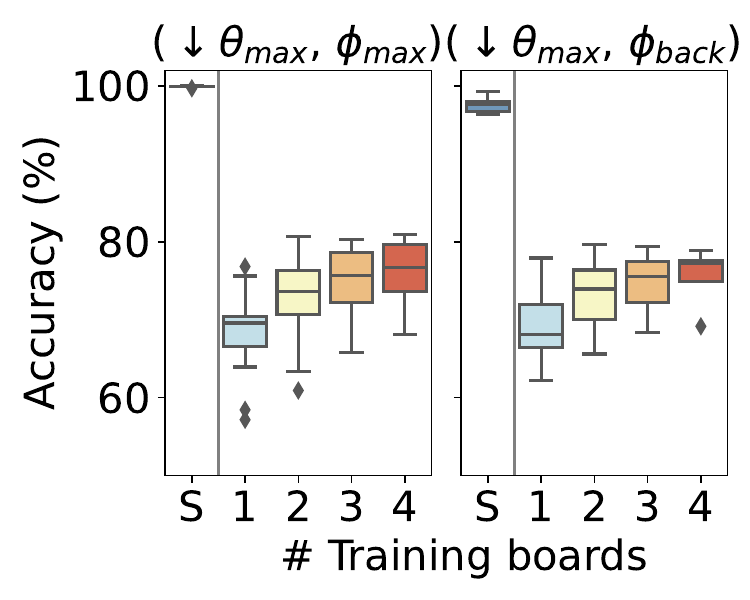
\includegraphics[width=0.90\linewidth]{fig/combo-nobacksub-and-backsub-acc-big.png}
  {\label{fig:multi-board-acc}}
\end{minipage}%
\begin{minipage}{.5\textwidth}
  \centering
  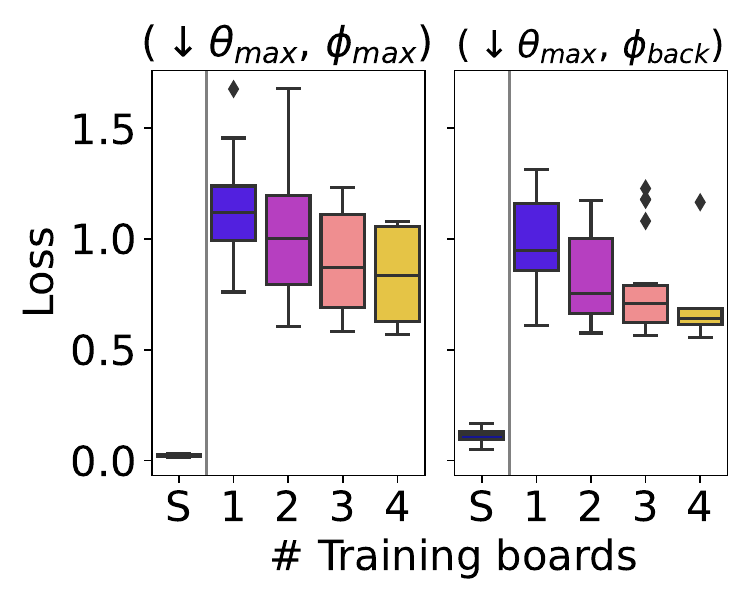
\includegraphics[width=0.90\linewidth]{fig/combo-nobacksub-and-backsub-loss-big.png}
  {\label{fig:multi-board-loss}}
\end{minipage}
\vspace{-10pt}
% \subfigure%[\hspace{15pt}Accuracy Boxplot]
% {\label{fig:multi-board-acc}
% \vspace{-50pt}
% 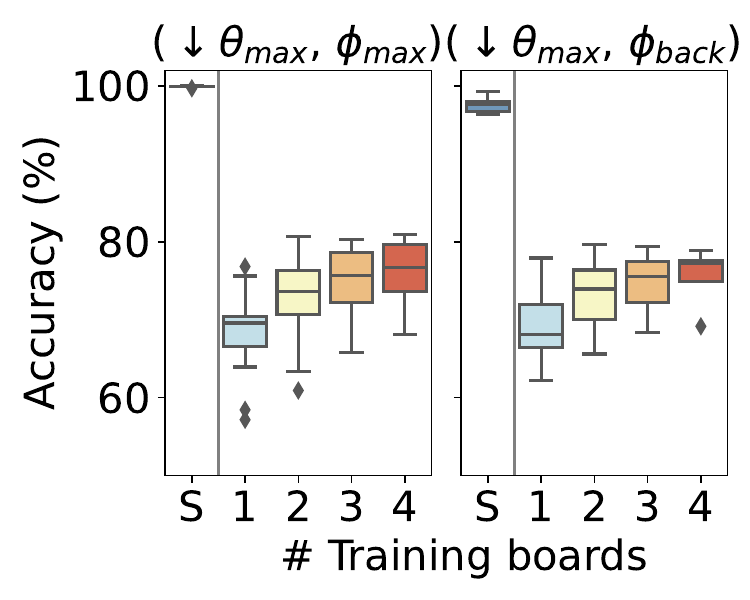
\includegraphics[width=0.55\columnwidth]{fig/combo-nobacksub-and-backsub-acc-big.png}
% }\\
% \vspace{-15pt}
% \subfigure%[\hspace{12pt}Loss Boxplot]
% {\label{fig:multi-board-loss}
% 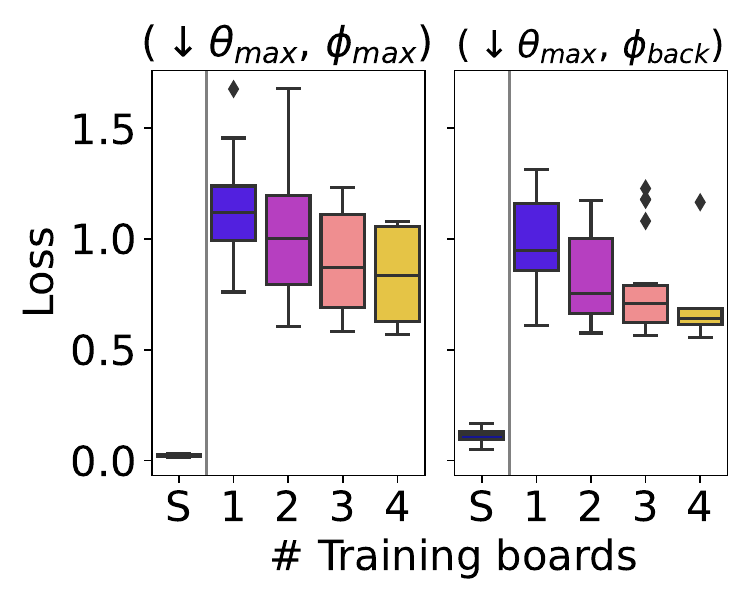
\includegraphics[width=0.55\columnwidth]{fig/combo-nobacksub-and-backsub-loss-big.png}}
% \vspace{-20pt}
\caption{Multi-board Training and Inference Results. Plots show Accuracy and Loss when training on 1-4 boards with background subtraction ($\downarrow\theta_{max}$, $\phi_{back}$) and without ($\downarrow\theta_{max}$, $\phi_{max}$). 
Testing always occurs on data from a separate board, except for when data from the same board is used (denoted ``S''). Background subtraction decreases the cross-board accuracy's interquartile range (IQR) by 2.3$\times$ and the loss's IQR by 5.8$\times$. 
Multi-board training and background subtraction greatly improve cross-board generalization.} 
\label{fig:multi-board}
\vspace{-10px}
\end{figure*}


After recognizing a cryptographic core with our classification procedure, we launch a Correlation Power Analysis (CPA)
attack \cite{brier04_correlation} to extract the key values. Because the values affect power consumption during encryption \cite{schellenberg2018inside}, our tuning techniques decrease the number of traces needed to extract the key.

\subsubsection*{\textbf{Maximizing Trace Information: }} 
CPA attack efficiency is dependent on both the quality of the measured power traces and on the CPA attack parameters used to construct a hypothetical power model \cite{krautter2019active, kar2018reducing, yu2017lightweight, mestiri2013comparative}. The selection of a power model and attack point for a CPA attack is dependent on the architecture of the co-tenant computation \cite{mestiri2013comparative}. The optimal attack parameters may be determined during the post-processing of measured traces and are dependent on the identified encryption algorithm implementation (Section \ref{classification}). Conversely, the quality of the measured power trace is influenced by the measurement signal-to-noise ratio which cannot be improved after trace collection \cite{krautter2019active, kar2018reducing, yu2017lightweight}. If the \sensor is not adequately tuned, the attack efficiency will be dramatically reduced. Our tuning techniques demonstrated in Sections \ref{capture_clock_tuning} and \ref{target_clock_tuning} improve the quality of measured power traces. We now demonstrate that for identical AES CPA attacks (i.e. identical power model and attack point), optimizing  $\phi$ and $\theta$ significantly improves the attack efficiency.

% After recognizing a cryptographic core with our classification procedure, we launch a Correlation Power Analysis (CPA) attack~\cite{brier04_correlation} to extract the key values from an AES computation. \textcolor{red}{Because the key values affect power consumption during encryption, prior work has demonstrated that \sensors can be used to perform key recovery \cite{schellenberg2018inside}.}
% %our tuning techniques decrease the number of traces needed to extract the key
% \textcolor{red}{Our tuning techniques improve these results by optimizing the information measured in each sample of a trace. }

%To evaluate the benefits of tuning, we perform this attack using different sensor configurations. CPA attacks can recover a cryptographic key from voltage fluctuation traces while the victim performs multiple AES encryption operations. As previously observed~\cite{schellenberg2018inside}, voltage fluctuations detected by TDCs depend on the value of the secret key, so measuring the voltage fluctuations enables an attacker to infer information about the key.

%In a CPA attack, the collected traces are first aligned so that a particular moment of the AES encryption computation appears at the same offset of all time-series trace data. Next, a leakage model is used to hypothesize how the voltage fluctuations should vary with different guesses for the unknown key bytes. The guessed key bytes are likely correct if the hypothesized fluctuations correlate with the measured fluctuations. In practice, the traces are noisy, so it takes several thousand traces for the computed correlation of the correct hypothesis to be more significant than the correlation of the incorrect hypotheses. The greater the signal-to-noise ratio of the trace data, the fewer traces are required for successful recovery. In the most basic attack against AES-128, each of the 16 ``subkey'' bytes in the key are considered independently. With 256 possible values for each subkey, this leads to an efficient key recovery method.

%\begin{comment}
\subsubsection*{\textbf{Setup:}}
We perform our CPA attack on the PYNQ-Z2 Orca AES application and consider the configurations ($\uparrow\theta_{max}$, $\phi_{back}$) for the well-optimized sensor and ($\uparrow\theta_{min}$, $\phi_{min}$) as a worst case un-tunable TDC comparison. The attack is repeated 50 times for each tuning strategy. We randomly generate a 128-bit AES key each time the attack is performed. This key is used by the Orca AES application to encrypt 50000 randomly generated plaintexts known to the attacker. During the encryption of each plaintext, the attacker collects a trace of length 8192, aligned by the measurement setup, so the beginning of the trace coincides with the beginning of the encryption. 

A large body of work exists on performing attacks on reducing traces needed~\cite{clavier14_practical}, alignment methods \cite{oswald2011breaking, van2011improving, gebotys2005analysis, plos2008evaluation}, or filtration methods~\cite{oswald13_side, ronen17_iot}. We have kept our CPA attack as conventional as possible for a fair comparison of the different sensor configurations.

%The leakage model hypothesizes that the voltage fluctuation at some offset in the trace correlates with $HW(SBox[k_i \oplus p_i])$, the hamming weight of the internal cipher state after the first substitution box step.

%We intentionally make conservative choices for the analysis, and we recognize that more advanced strategies lead to key recovery in fewer traces~\cite{clavier14_practical}. 
%A real-world attack such as \cite{oswald2011breaking} would involve some alignment method~\cite{van2011improving,gebotys2005analysis,plos2008evaluation} or further filtering of collected traces~\cite{oswald13_side,ronen17_iot}.
%Indeed, we implemented some common strategies and found them helpful in recovering the full key. However, opting for a particular processing technique could bias the results if its effectiveness depends on the variance of the source trace. We have therefore kept the CPA attack as conventional as possible for a fair comparison of the different sensor configurations.
%\end{comment}

Following prior work, we analyze the results of the CPA attacks using multiple metrics~\cite{clavier14_practical}. After processing some traces, the CPA method returns a list for each subkey that ranks the possible subkey values from most likely to least likely. Partial Guessing Entropy (PGE) is the position of the correct subkey value in the list, where lower is better. Partial Success Rate (PSR) is the frequency with which the correct subkey value is ranked as most likely. Global Success Rate (GSR) is the frequency with which all correct subkey values are ranked as most likely. We also consider the mean PGE as a function of the number of traces. This is frequently used to compare the performance of CPA attacks~\cite{oflynn15_side,oflynn16_power,oflynn19_device}.

\subsubsection*{\textbf{CPA Attack Results:}}
%\begin{table}[ht!]
%\centering
%\caption{Evaluation of CPA attack performance.}\label{table:cpastats}

%\begin{tabular}{rcc}
%Metric                                 & ($\uparrow\theta_{max}$, %$\phi_{back}$) & ($\uparrow\theta_{min}$, $\phi_{min}$)  \\
%\hline
%GSR @ 50k & 5\% & 0\% \\
%PSR @ 50k & (15\%, 48\%, 90\%) & (5\%, 23\%, 45\%) \\
%PGE @ 50k & (0.8, 46.9, 95.4) & (54.8, 87.2, 126.2)
%\end{tabular}
%\end{table}
Our results demonstrate that the optimized sensor configuration ($\uparrow\theta_{max}$, $\phi_{back}$) outperforms the worst-case of an un-tunable sensor ($\uparrow\theta_{min}$, $\phi_{min}$). Qualitative results are given in Figure~\ref{fig:mean-pge}, which show that the traces obtained from ($\uparrow\theta_{max}$, $\phi_{back}$) exhibit lower PGE on average. This indicates that fewer traces are needed to recover the key when using the ($\uparrow\theta_{max}$, $\phi_{back}$) configuration, lowering the overall cost of the attack.

Numerical (Min, Avg, Max) results are given in Table~\ref{table:cpastats}. The GSR statistic shows that the optimized sensor configuration ($\uparrow\theta_{max}$, $\phi_{back}$) was able to recover all 16 subkeys in a single trial. In contrast, a poorly tuned sensor ($\uparrow\theta_{min}$, $\phi_{min}$) never recovered the entire key. The higher PSR values for the well-tuned sensor demonstrate that individual subkeys were recovered around 2$\times$ more frequently given the same number of traces as with a poorly tuned sensor. These results show that optimized sensor configuration is crucial for identifying co-tenant computation and significantly increases the rate at which a cryptographic key can be recovered.

\begin{figure}[t]
\centering
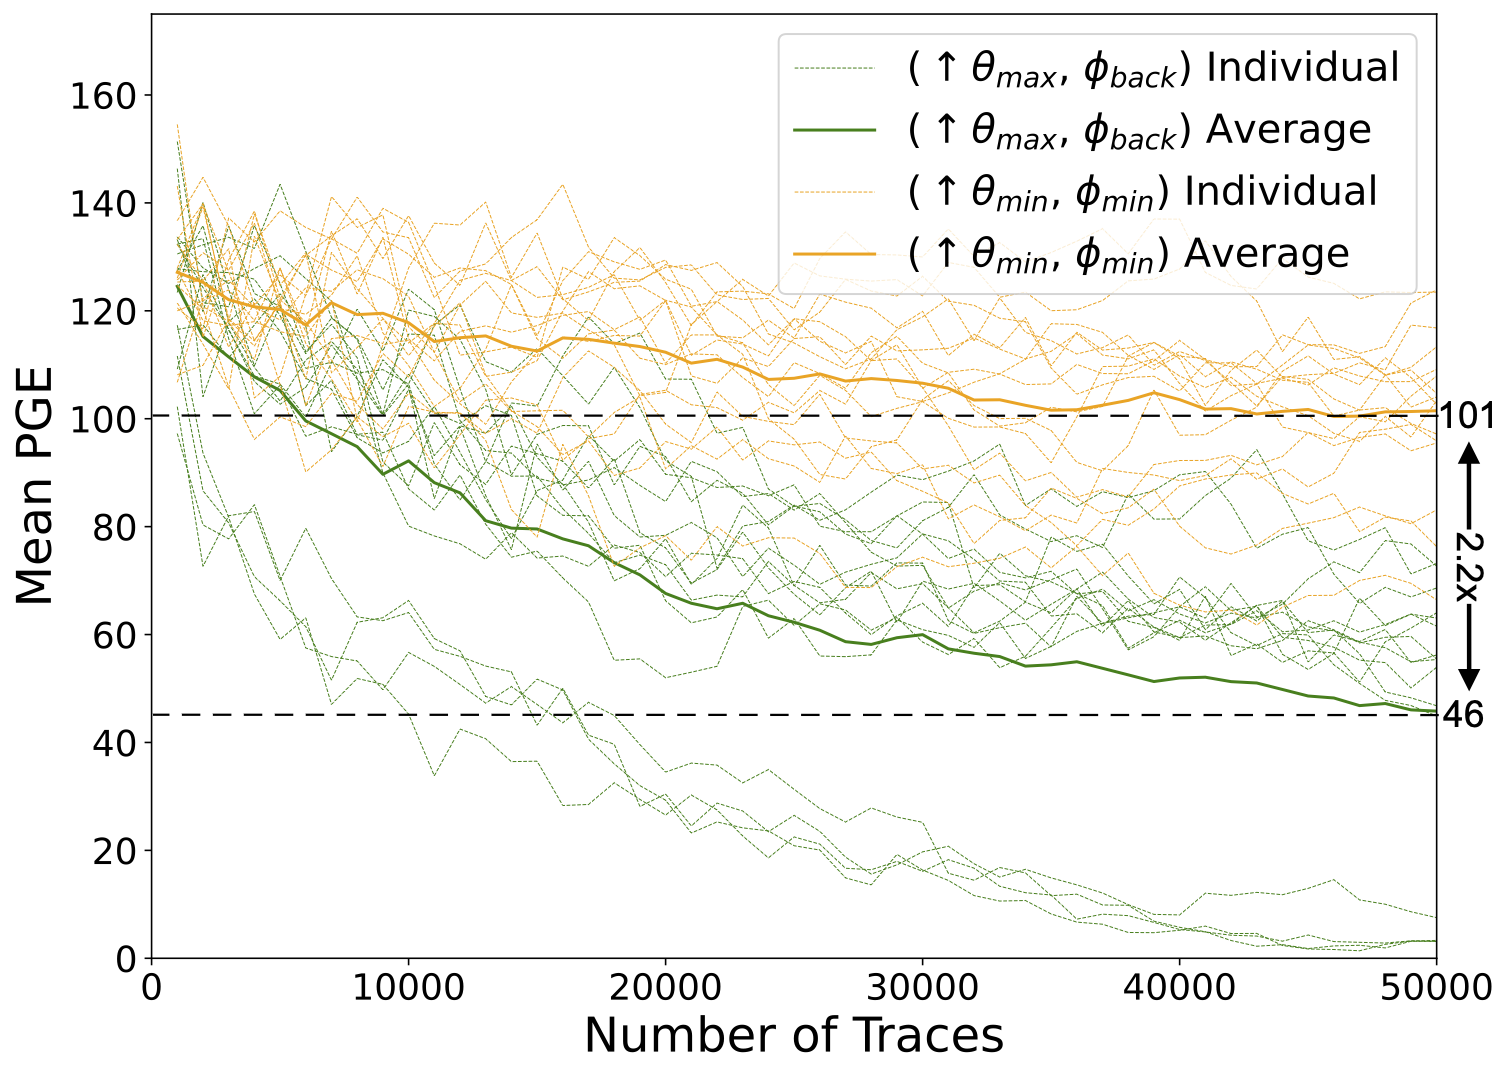
\includegraphics[width= 0.6\linewidth]{img/mean_pge_vs_traces.png}\\
\vspace{-10px}
\caption{Performance of a CPA attack for ($\uparrow\theta_{max}$, $\phi_{back}$) and ($\uparrow\theta_{min}$, $\phi_{min}$) tuning parameters. Lower average PGE indicates that the attack is performing better, as the correct subkey values are ranked as more likely after processing fewer traces. Our tuning method has a significant impact on key recovery, lowering PGE by 2.2$\times$ at 50,000 traces.}
\label{fig:mean-pge}
\vspace{-12px}
\end{figure}

%Again, we emphasize that the absolute performance according to these metrics is not the goal of this evaluation. Instead, we use the relative performance to compare two sensor configuration strategies. The ($\uparrow\theta_{max}$, $\phi_{back}$) tuning strategy yields traces that are more effectively processed in a CPA attack than the ($\uparrow\theta_{min}$, $\phi_{min}$) tuning strategy.

%\end{comment}
